\chapter{Reinforcement Learning}\label{chap:RL}
Reinforcement learning is a machine learning method approach concerned with  optimal action selection based on current state. 
In this chapter a computational approach to learning through interactions with an environment is presented. The majority of information gathered is sourced to Sutton and Bartos \textit{Reinforcement Learning - An Introduction} \cite{Sutton2020} and this chapter can be seen as a preliminary chapter which can be skipped if the reader is well informed within the topic of both tabular and function approximation reinforcement learning methods.

\newpage

\section{Introduction to Reinforcement Learning}\label{sec:introRL}
As discussed in \cref{sec:introMotivation} this project will focus on the application of the model-free method called reinforcement learning. \cref{fig:Agent-environment} presents the basic structure of reinforcement learning and elements involved. There are two actors in the reinforcement learning framework, the \textit{agent}, and the \textit{environment}. 

\begin{figure}[h!]
	\centering
	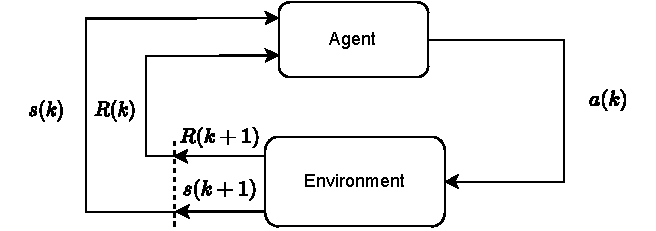
\includegraphics[width=1\linewidth]{Figures/AgentEnvironment.pdf}
	\caption{Interactions between agent and environment.}
	\label{fig:Agent-environment}
\end{figure}

The agent applies control action $ a(k) $ to the environment, based on the current state-combination $ s(k) $ and receives reward $ R(k+1) $, for bringing the environment to a new state $ s(k+1) $. The process is repeated until the state is terminal. The reinforcement learning sequence is: 

\begin{equation}
	s(0), a(0), R(1), s(1), a(1), R(2), s(2), a(2),\cdots	
\end{equation}

For discrete state and discrete action reinforcement learning: $ a(k)\in \mathcal{A} $, $s(k)\in \mathcal{S} $. That is, the available states and actions belongs to closed sets $\mathcal{S,A}$. And the reward $ R(k+1) \in \mathcal{R} \subset \mathbb{R} $. Notice that we take some notational freedom here, and exclude $s$ and $a$ from the $R$ notation, $R$ does inherently depend on state and action.

The agent seeks to maximise a series of rewards over time, called return $(G)$, through choices of actions \cite{Sutton2020}. Often a weighted sum of reward is used with $0 \leq \gamma \leq 1$:

\begin{equation}\label{eq:ExpectedReturn1}
	G(k)=R(k+1)
	+\gamma R(k+2)
%	+\gamma^{2}R(k+3)
	+\cdots
	+\gamma^{m}R(k+m+1)
	=\sum_{n=0}^{m}\gamma^{n}R(k+n+1)
\end{equation}

Where $ m $ is final time step of learning. In some problems learning is continuing and $m = \infty$. Learning problems with finite $m$ are called \textit{episodic}. This project deals with continuing learning, and we will use infinity throughout the report. 

By choosing $0 \leq \gamma < 1$ it ensures that higher importance is given to immediate reward rather than future rewards. Rewriting \cref{eq:ExpectedReturn1} to a recursive form yields:

\begin{equation}\label{eq:ExpectedReturn2}
	\begin{split}
			G(k)&=R(k+1)+\gamma R(k+2)+\gamma^2 R(k+3)+\cdots\\
			    &=R(k+1)+\gamma\big(R(k+2)+\gamma R(k+3)+\cdots\big)\\
			    &=R(k+1)+\gamma G(k+1)
	\end{split}
\end{equation}

The value function is defined as the expected return under a policy $ \mathbb{E}_{\pi} $, when starting in $a(k)$ state $ s(k) $ and afterwards following a policy $ \pi $ and is a measure of the \textit{value} of being in a state.   

%\begin{equation}\label{eq:IntroVfunc}
%		v_{\pi}(s)=\mathbb{E}_{\pi}\bigg[ %G(k) \big| s(k)=s\bigg]
%		%=\mathbb{E}_{\pi}\bigg[=R(k+1)+\gamma %G(k+1) \big| s(k)=s\bigg]
%\end{equation}

\begin{equation}\label{eq:IntroVfunc}
	v_{\pi}\bigg(s(k)\bigg)=\mathbb{E}_{\pi}\bigg[ G(k) \; \big|  \; s(k)\bigg]
	=\mathbb{E}_{\pi}\bigg[=R(k+1)+\gamma G(k+1) \; \big| \; s(k)\bigg]
\end{equation}

The policy $ \pi $ determines control actions, that is a mapping of the current state into an action - $ s(k) \mapsto a(k) $. $\pi$ is usually designed such that it selects actions resulting in highest expected return. Such a policy results in the optimal value-function:

%\begin{equation}
%	v_{\star}(s)=\underset{\pi}{\max} \; v_{\pi}(s)
%\end{equation}

\begin{equation}
	v_{\star}\bigg(s(k)\bigg)=\underset{\pi}{\max} \; v_{\pi}\bigg(s(k)\bigg)
\end{equation}

Since it is not realistic to maximise over all possible policies, we introduce the action value function in the pursuit of finding a different approach. The action value function is defined as the expected return when taking an action $ a(k) $ in a state $s(k)$ and afterwards following policy $\pi$:

%\begin{equation}\label{eq:IntroQfunc}
%	Q_{\pi}(s,a)=\mathbb{E}_{\pi}\bigg[ G(k) \big| s(k)=s,a(k)=a \bigg]
%	=\mathbb{E}_{\pi}\bigg[ R(k+1)+\gamma G(k+1) \big| s(k)=s,a(k)=a\bigg]
%\end{equation}

\begin{equation}\label{eq:IntroQfunc}
	Q_{\pi}\bigg(s(k),a(k)\bigg)=\mathbb{E}_{\pi}\bigg[ G(k) \; \big| \; s(k),a(k) \bigg]
	=\mathbb{E}_{\pi}\bigg[ R(k+1)+\gamma G(k+1) \; \big| \; s(k),a(k)\bigg]
\end{equation}

Optimal policies share same optimal action value functions which are defined as:

%\begin{equation}
%	Q_{\star}\bigg(s,a\bigg)=\underset{\pi}{\max} \; Q_{\pi}\bigg(s,a\bigg)
%\end{equation}

\begin{equation}
	Q_{\star}\bigg(s(k),a(k)\bigg)=\underset{\pi}{\max} \; Q_{\pi}\bigg(s(k),a(k)\bigg)
\end{equation}

$ Q_{\star} $ can be written in terms of $ v_{\star} $:

%\begin{equation}
%	Q_{\star}\bigg(s,a\bigg)=\mathbb{E}\bigg[R(k+1)+\gamma v_{\star}\bigg(s(k+1)\bigg) \big| s(k)=s,a(k)=a \bigg]
%\end{equation}

\begin{equation}
	Q_{\star}\bigg(s(k),a(k)\bigg)=\mathbb{E}\bigg[R(k+1)+\gamma v_{\star}\bigg(s(k+1)\bigg) \; \big| \; s(k),a(k) \bigg]
\end{equation}

This function computes the expected return for taking action $a(k)$ while being in state $s(k)$, and afterwards following an optimal policy. The entire value of following an optimal policy is contained in the optimal state value of the next state.

The optimal value of a state under an optimal policy must equal the expected return for the best action from that state. This action can be found by finding the action that yields the maximum value in the action value function.

%\begin{equation}
%	\begin{split}
%		v_{\star}\bigg(s\bigg)&=\underset{a'}{\max} \; Q_{\pi\star}\bigg(s,a'\bigg)\\
%					&=\underset{a'}{\max} \; \mathbb{E}_{\pi\star}\bigg[ R(k+1)+\gamma G(k+1) \big| s(k)=s,a(k)=a'\bigg]\\
%					&=\underset{a'}{\max} \; \mathbb{E}\bigg[ R(k+1)+\gamma v_{\star}\bigg(s(k+1)\bigg) \big| s(k)=s,a(k)=a'\bigg]\\
%					&=\underset{a'}{\max}\sum_{s'}p\bigg(s'|s(k),a'\bigg)\bigg[R(k+1)+\gamma v_{*}(s')\bigg]
%		\end{split}
%\end{equation}

\begin{equation}
	\begin{split}
		v_{\star}\bigg(s(k)\bigg)&=\underset{a'}{\max} \; Q_{\pi\star}\bigg(s(k),a'\bigg)\\
		&=\underset{a'}{\max} \; \mathbb{E}_{\pi\star}\bigg[ R(k+1)+\gamma G(k+1) \; \big| \; s(k),a'\bigg]\\
		&=\underset{a'}{\max} \; \mathbb{E}\bigg[ R(k+1)+\gamma v_{\star}\bigg(s(k+1)\bigg) \; \big| \; s(k),a'\bigg]\\
		&=\underset{a'}{\max}\sum_{s'}p\bigg(s' \; \big| \; s(k),a'\bigg)\bigg[R(k+1)+\gamma v_{*}(s')\bigg]
	\end{split}
\end{equation}

Where $ p(s'|s,a) $ is  probability of transition to state $ s' $, from state $ s(k) $ taking action $ a' $. The last equation is the Bellman optimality equation, see the next \cref{sec:Bellman}. Similarly the Bellman equation for the action value function can be written as:

%\begin{equation}
%	\begin{split}
%		Q_{\star}\bigg(s,a\bigg)&=\mathbb{E}\bigg[R(k+1) + \gamma \underset{a'}{\max} \; Q_{\star}\bigg(s(k+1),a'\bigg)\big|s(k)=s,a(k)=a\bigg]\\
%		&= \sum_{s'}p\bigg(s'|s(k),a(k)\bigg)\bigg[R(k+1)+\gamma \max_{a'}Q_{*}\bigg(s',a'\bigg)\bigg]
%	\end{split}
%\end{equation}

\begin{equation}
	\begin{split}
		Q_{\star}\bigg(s(k),a(k)\bigg)&=\mathbb{E}\bigg[R(k+1) + \gamma \underset{a'}{\max} \; Q_{\star}\big(s(k+1),a'\big) \; \big| \; s(k),a(k)\bigg]\\
		&= \sum_{s'}p\bigg(s'|s(k),a(k)\bigg)\bigg[R(k+1)+\gamma \max_{a'}Q_{*}\big(s',a'\big)\bigg]
	\end{split}
\end{equation}
 
\newpage

\section{The Bellman Equation} \label{sec:Bellman}
Here a more detailed look at the Bellman equation in its general from is presented. It lays the foundation for reinforcement learning solutions.  

\begin{equation}\label{eq:Bellman}
	v_{\pi}\bigg(s(k)\bigg)=\sum_{a'}\pi\bigg(a'|s(k)\bigg)\sum_{s'}p\bigg(s'|s(k),a'\bigg)\bigg[R(k+1)+\gamma v_{\pi}(s')\bigg]
\end{equation}

where,
\begin{center}
	\begin{tabular}{l p{12cm}}
		$v_{\pi}\bigg(s(k)\bigg) $ & is the  value of state $ s(k) $ under policy $ \pi $\\ 
		$ \pi\bigg(a'|s(k)\bigg) $ & is the conditional probability of taking action $ a' $ in state $ s(k) $ under stochastic policy $ \pi $\\
		$ p\bigg(s'|s(k),a'\bigg) $ & is the conditional probability of transitioning to state $ s' $ when taking action $ a' $ in state $ s(k) $ \\
%		$R(k+1)$ & is the reward for bringing the environment from $ s(k) \rightarrow s(k+1) $\\
	\end{tabular}
\end{center}

\hfill 

\cref{eq:Bellman} is the Bellman equation for the value function. The equation can be read as weighing the immediate reward and a discounted version of future state value by the probability of getting that reward and next state, when taking a specific action in a given state.  When summing over all possible actions and their possible next states an expression for the expected value of being in that state is obtained. In some versions of \cref{eq:Bellman} you also sum over all possible rewards, however, we assume it to be deterministic.

These optimality equations make systems of equations which can be solved, this is the Dynamic Programming approach. However, the set of equations are potentially unsolvable, and require a complete model of the system to know the transition probabilities. Therefore \cref{sec:TD-Methods} considers model-free estimation methods \textit{SARSA} and \textit{Q-learning}.

\section{Policies}

The simplest policy chooses actions based on the highest expected return achievable in a state $ s(k) $, that is, the highest action value:

\begin{equation}\label{eq:Greedy}
	a(k)=\underset{a'\in \mathcal{A}}{\arg\max} \; Q\bigg(s(k),a'\bigg)
\end{equation}

\cref{eq:Greedy} is called the \textit{greedy-policy}. The policy clearly takes advantage of already known information about the action values, this is known as \textit{exploitation}.

A greedy policy always chooses the action that it thinks is best at the current time, but this may result in convergence to a sub-optimal policy. The algorithm can get tunnel vision on a specific policy if it never checks other options, options which might yield better returns, especially in the long run. For example scenarios where multiple bad steps must be taken before a big reward is achieved. A greedy policy is also not able to detect changes in the environment. Allowing the agent to \textit{explore} new knowledge about the action value function can improve the agent's knowledge and lead to better decision making and performance. \cref{eq:EpsilonGreedy} presents the \textit{Epsilon-Greedy policy} which is a very simple method that balances exploration and exploitation by randomly choosing between the two options:

\begin{equation}\label{eq:EpsilonGreedy}
	a(k) = 
	\begin{cases} 
		\underset{a'\in \mathcal{A}}{\arg\max} \; Q\bigg(s(k),a'\bigg) & \text{exploitation with probability} \; 1-\epsilon  \\
		\text{Random action from $ \mathcal{A} $} & \text{exploration with probability} \; \epsilon 
	\end{cases},\quad \epsilon \in [0,1]
\end{equation}

If the $\epsilon$-value is chosen low \cref{eq:EpsilonGreedy} behaves greedy most of the time, but sometimes, instead of following the greedy-policy, it randomly chooses an action from the closed set of actions with equal probability independent of best action value. Doing this means the entire state-action space is explored as $ k \rightarrow \infty $. The downside is the immediate loss of reward from randomly choosing a worse action, this is especially noticeable as the algorithm gets closer to convergence, and shows the diminishing effectiveness of exploration.	

\section{Temporal Difference Methods}\label{sec:TD-Methods}
We choose to skip the topic of Monte Carlo simulation, as we wish to avoid its disadvantage of batch updating  - see e.g. \cite{Busoniu2010, Sutton2020} - and go directly to the topic of Temporal Difference learning. Temporal difference learning is a central idea of reinforcement learning. It makes it possible for the agent to learn while interacting with the environment for which no knowledge about the dynamics is known \cite{DaMottaSallesBarreto2008}, and in an iterative way finds the optimal action value function. It is also proven to converge to an optimal policy under the same conditions as other methods, and although temporal difference methods has not been proven to converge faster mathematically, empiric experiments show that temporal difference methods converge faster than Monte Carlo methods \cite{Sutton2020}.

SARSA is an abbreviation of State-Action-Reward-State-Action and forms the basis of TD(0) learning:

\begin{equation}\label{eq:sarsa}
	Q\bigg(s(k),a(k)\bigg)\leftarrow Q\bigg(
	s(k),a(k)\bigg)+\alpha	 
	\Bigg[
	\underbrace{R(k+1)+\gamma Q\bigg(s(k+1),a(k+1)\bigg)}_{\text{Temporal difference target/Sarsa target}}
	-Q\bigg(s(k),a(k)\bigg)
	\Bigg]
\end{equation}

Unlike Monte Carlo methods, Temporal Difference learning updates an action value after every iteration. This results in least amount of time spent on making sub-optimal actions. The method updates an estimate of the action value function based on the same estimate. This is called bootstrapping. 

Temporal Difference methods use \textit{sample updates} and therefore does not require a system model. This means looking ahead and combining the value at the next state-action pair and the reward obtained along the way, to compute a backed-up value for the current iteration (k), which is used to update the original state \cite{Sutton2020}.

One of the most used reinforcement learning method is called Q-learning, which like \cref{eq:sarsa} approximates the Bellman equation by updating the action value function iteratively  as seen in \cref{eq:Q-learning}.

\begin{equation}\label{eq:Q-learning}
	Q\bigg(s(k),a(k)\bigg)\leftarrow Q\bigg(s(k),a(k)\bigg)+\alpha \Bigg[
	\underbrace{R(k+1)+\gamma \max_{a'} 
		Q\bigg(s(k+1),a'\bigg)}_{\text{Q-Learning target}}
	-Q\bigg(s(k),a(k)\bigg)
	\Bigg]
\end{equation}

where,
\begin{center}
	\begin{tabular}{l p{12cm}}
		$ \alpha $ & is the \textit{Learning rate}. $0\leq \alpha \leq 1$. \\
	\end{tabular}
\end{center}

Note that the only difference in the two update methods lies in the target. This difference is called \textit{on-} and \textit{off-} policy, depending on whether the update is based on strictly staying on policy, meaning target action is selected according to policy (SARSA), or target action is chosen optimally, independent of policy (Q-learning). This essentially means that Q-learning converges to the optimal policy immediately, where SARSA converges to a less optimal policy which also consider the randomness of the $ \epsilon$-greedy policy, such that a \textit{safer} policy is obtained. Here safety means policies in which random actions can lead to large negative reward, achieve less value.

The learning rate $\alpha$ dictates the size of updates, but also affects if the algorithm can converge at all. The following properties on $ \alpha $ grantees convergence \cite{Busoniu2010}, such that if: 

\begin{equation}\label{eq:alphaAssumptions}
	\sum_{k=1}^{\infty}\alpha(k)=\infty \quad \wedge \quad \sum_{k=1}^{\infty}\alpha(k)^{2}<\infty
\end{equation} 

Then: 

\begin{equation}
	Q(s,a) \rightarrow Q_\star(s,a)\hspace{0.108cm} \text{as}\hspace{0.108cm}k \rightarrow\infty,\hspace{0.108cm} \forall s,a \in \mathcal{S,A}
\end{equation}

Where $ Q_{\star} $ denotes the optimal action value function. The first condition in \cref{eq:alphaAssumptions} is required to guarantee that the steps are large enough to eventually
overcome any initial conditions or random fluctuations. The second condition guarantees
that eventually the steps become small enough to assure convergence \cite{Sutton2020}.

\section{Function Approximation}\label{sec:FuncApprox}
One way of keeping track of the action values is to use a table. For large systems with high state-action dimensionality this is not desirable. The agent is required to visit all state-action combinations at least once to get an idea of optimal decision making. Visiting the whole state-action space could take an enormous amount of time resulting in long learning periods and convergence times.

Instead the action value function can be approximated \cite{Sutton2020}. This allows us to generalise information about visited state-actions pairs to not yet visited pairs:

\begin{equation}\label{eq:QApprox1}
	\hat{Q}\bigg(s(k),a(k),\textbf{w}\bigg) \approx Q_{\pi}\bigg(s(k),a(k)\bigg)
\end{equation}

The state-action function estimate is now represented as a parametrised function form with a weight vector $ \textbf{w} \in \mathbb{R}^{d}$. The linear\footnote{Linear with respect to weights} approximation of the action-value function is given by:

\begin{equation}\label{eq:QApprox2}
	\hat{Q}\bigg(s(k),a(k),\textbf{w}\bigg)=\textbf{w}^{\intercal}\textbf{x}\bigg(s(k),a(k)\bigg)=\sum_{i=1}^{d}w_{i}x_{i}\bigg(s(k),a(k)\bigg)
\end{equation}

Where 

\begin{equation}
	\textbf{x}\bigg(s(k),a(k)\bigg) = \bigg[x_{1}\bigg(s(k),a(k)\bigg), x_{2}\bigg(s(k),a(k)\bigg) \cdots x_{d}\bigg(s(k),a(k)\bigg)\bigg]^\intercal
\end{equation}
 
is the feature vector and each element $ x_{i} $ is called a feature of the states.

The weight vector is updated using stochastic gradient descent, which minimises the squared error between the true state-action function and the estimated function \cite{Overgaard2019}:

\begin{equation}\label{eq:QApprox3}
	\begin{split}
		\textbf{w} 
		& \leftarrow\textbf{w}-\frac{1}{2}\alpha\nabla_{\textbf{w}}\big[Q_{\pi}\bigg(s(k),a(k)\bigg)-\hat{Q}\bigg(s(k),a(k),\textbf{w}\bigg)\bigg]^{2}\\
		&=\textbf{w}+\alpha\bigg[Q_{\pi}\bigg(s(k),a(k)\bigg)-\hat{Q}\bigg(s(k),a(k),\textbf{w}\bigg)\bigg]\nabla_{\textbf{w}}\hat{Q}\bigg(s(k),a(k),\textbf{w}\bigg)
	\end{split}
\end{equation}


$\alpha$ is a positive step size, and $\nabla_{\textbf{w}} \hat{Q}\bigg(s(k),a(k),\textbf{w}\bigg)$ is the gradient of the function $ \hat{Q} $ with respect to the weight vector $ \textbf{w} $. \cref{eq:QApprox3} requires that the actual action value function $ Q_{\pi} $ is known which is typically not the case. An estimate, $ U $, of $ Q_{\pi}\bigg(s(k),a(k)\bigg) $ is used:

\begin{equation}\label{eq:QApprox5}
	\textbf{w}_{} \leftarrow \textbf{w}_{}+\alpha\bigg[U-\hat{Q}\bigg(s(k),a(k),\textbf{w}\bigg)\bigg]\nabla\hat{Q}\bigg(s(k),a(k),\textbf{w}\bigg)
\end{equation}

Choosing the estimate as in \cite{Overgaard2019,Sutton2020}: 

\begin{equation}\label{eq:SSGDtarget}
	U = R(k+1)+\gamma \max_{a'}\hat{Q}\bigg(s(k+1),a',\textbf{w}\bigg)
\end{equation}

Combining \cref{eq:QApprox5} and \cref{eq:SSGDtarget} yields the update law for the weight vector:

\begin{equation}\label{eq:QApprox6}
	\textbf{w} \leftarrow \textbf{w}
	+\alpha\bigg[R(k+1)+\gamma\max_{a'}\hat{Q}\bigg(s(k+1),a',\textbf{w}\bigg)
	-\hat{Q}\bigg(s(k),a(k),\textbf{w}\bigg)\bigg]\nabla_{\textbf{w}}\hat{Q}\bigg(s(k),a(k),\textbf{w}\bigg)
\end{equation}

Evaluating $ \nabla_{\textbf{w}}\hat{Q}\bigg(s(k),a(k),\textbf{w}\bigg) $ in \cref{eq:QApprox2} yields:

\begin{equation}\label{eq:NablaQApprox}
\begin{split}
		\nabla_{\textbf{w}}\hat{Q}\bigg(s(k),a(k),\textbf{w}\bigg) 
		&=\nabla_{\textbf{w}}\bigg(\textbf{w}^{\intercal}\textbf{x}\bigg(s(k),a(k)\bigg)\bigg)\\
	&=\textbf{x}\bigg(s(k),a(k)\bigg)
\end{split}
\end{equation}

\cref{eq:QApproxFinal} presents the semi-gradient descent update rule for function approximation: 

\begin{equation}\label{eq:QApproxFinal}
	\textbf{w} \leftarrow \textbf{w}
	+\alpha\bigg[R(k+1)+\gamma\max_{a'}\hat{Q}\bigg(s(k+1),a',\textbf{w}\bigg)
	-\hat{Q}\bigg(s(k),a(k),\textbf{w}\bigg)\bigg]\textbf{x}\bigg(s(k),a(k)\bigg)
\end{equation}

\newpage